\subsection{Implications for the Galactic Center Gamma-Ray Excess}


As stated in the introduction, very few pulsars have been detected in the vicinity of the Inner Galaxy. If the GCE is generated by MSPs, this fact requires the MSPs responsible for this signal to be faint enough to have gone undetected. This, in turn, would require the MSPs in the Inner Galaxy to be systematically lower in luminosity than those found in other environments~\cite{Holst:2024fvb} (see also, Refs.~\cite{Cholis:2014noa,Hooper:2016rap,Hooper:2015jlu,Bartels:2018xom,Ploeg:2017vai,Ploeg:2020jeh,Dinsmore:2021nip}).


\begin{figure}[t]
\centering
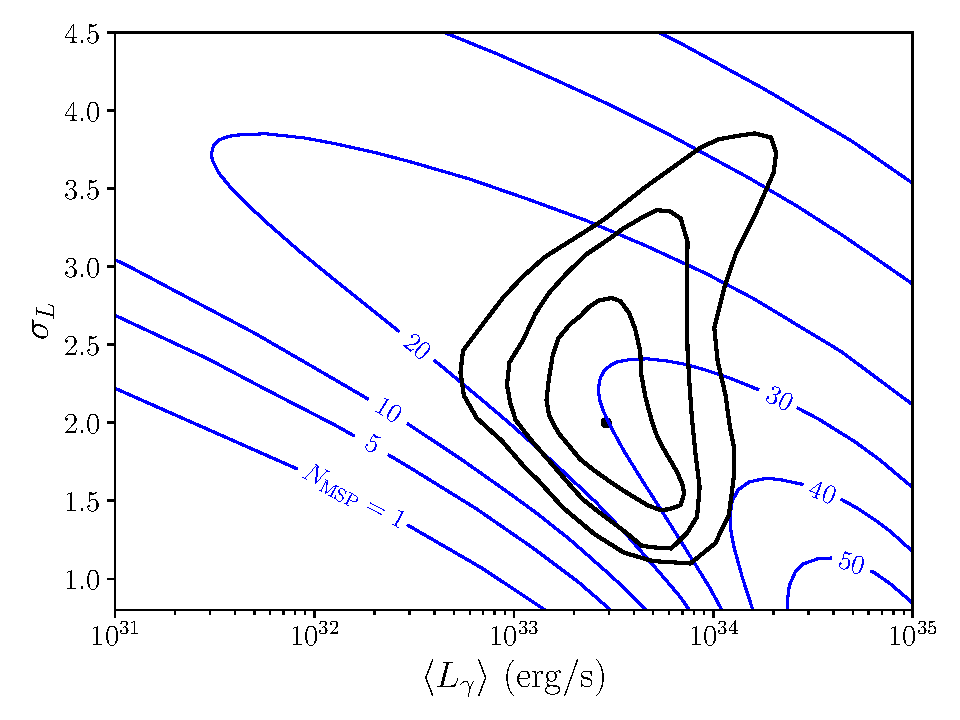
\includegraphics[width=0.66\textwidth]{sections/paper_msp/img/3PC.pdf}
\caption{The constraints on the MSP gamma-ray luminosity found in this study (shown for the case of $\langle N_\textrm{MSP}\rangle = R_\textrm{MSP}\, \Gamma_e^{0.7} +R'_\textrm{MSP} \,L_V$), shown along with contours representing the number of Inner Galaxy MSPs that should
appear in the Fermi source catalogs, $N_\textrm{MSP}$, assuming that the Galactic Center Gamma-Ray Excess (GCE) is generated by MSPs~\cite{Holst:2024fvb}. As there are only three Inner Galaxy pulsars candidates in the 3PC, MSPs can generate the excess
gamma-ray emission only if that source population consists of members that are significantly less luminous than those present in globular clusters.}
\label{fig:3PC}
\end{figure}



The possibility that the Inner Galaxy could contain a large population of low-luminosity pulsars has been motivated by the large proportion of old stars that are found in the Galactic Bulge relative to those in the Galactic Plane. The stellar populations found in globular clusters, however, are comparably old to those in the Bulge. By measuring the gamma-ray luminosity function of MSPs in globular clusters, we can hope to shed some light on the question of whether the Inner Galaxy might contain a very large abundance of very low-luminosity MSPs. 

In Fig.~\ref{fig:3PC}, we plot the number of MSPs that should have been detected by Fermi and contained within their source catalogs~\cite{Fermi-LAT:2023zzt} if they were responsible for producing the GCE, as a function of the luminosity function parameters~\cite{Holst:2024fvb}. If the GCE is generated by MSPs with the same luminosity function and other characteristics as those found in globular clusters, Fermi's source catalogs would have contained $N_\textrm{MSP}\sim 17-37$ individual members of this population. Given that only three millisecond pulsars have been detected with a direction and distance that does not preclude it from being part of an Inner Galaxy population, the luminosity function derived here is incompatible with pulsar interpretations of the GCE, unless a large number of unassociated Fermi sources are, in fact, unidentified MSPs. Given systematic efforts that have been conducted to search for radio pulsations from unassociated Fermi sources, this possibility seems unlikely. Alternatively, the observed gamma-ray excess could be generated by MSPs if those pulsars are significantly less luminous, on average, than those located in globular clusters or in the Galactic Plane. 

\begin{figure}[t]
\centering
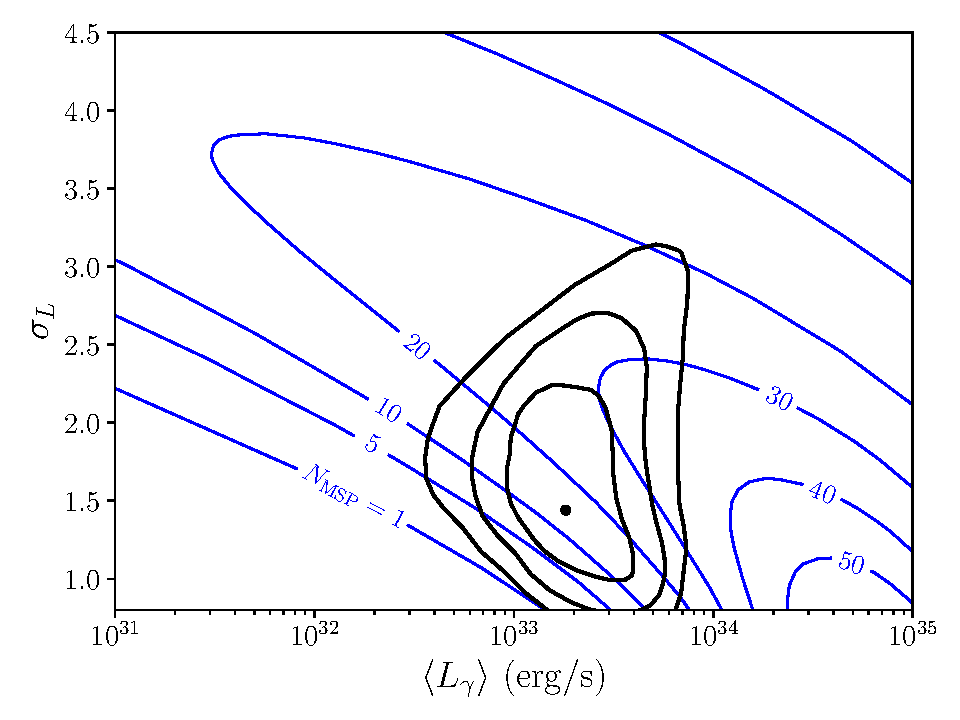
\includegraphics[width=0.66\textwidth]{sections/paper_msp/img/3PC-c2c-var.pdf}
\caption{ As in Figure \ref{fig:3PC}, but for the best fit model including cluster-to-cluster variations. The results are compatible with the estimates in Figure \ref{fig:3PC} within the $1\sigma$ band, although the model with cluster-to-cluster variations favors lower values for $\langle L_{\gamma} \rangle$ and $\sigma_L$.}
\label{fig:3PC-c2c-var}
\end{figure}

As mentioned in Section \ref{sec:glf}, our models for the mean number of millisecond pulsars in a given globular cluster are subject to intrinsic uncertainties. To account for this, we also considered a more flexible model that includes an intrinsic cluster-to-cluster variation in the expected number of MSPs. The purpose of this approach is to derive a more conservative lower bound on the number of pulsars that should have been detected in the Inner Galaxy if they are responsible for the Galactic Center Excess. In Figure \ref{fig:3PC-c2c-var}, we show the results of this analysis. By allowing for a wider range of pulsar populations, particularly those that are fainter on average, this model lowers the number of expected detections to the range of $N_\textrm{MSP} \approx 3 -30$.  Although this bound is less constraining by construction, the results nonetheless remain in tension at a level of at least $2\sigma$ with the three identified pulsar candidates.

